\begin{frame}{Estructura de bandas del $YCrO_{3}$}
    \begin{columns}[t]
        \column{0.5\textwidth}
        \begin{figure}[H]
            \centering
            \includegraphics[width=1.0\textwidth]{contenido/resultados/img_resultados/YCO_bandas_A.png}
            \caption{Bandas de energ\'ia del $YCrO_{3}$ con arreglo         
                antiferromagn\'etico tipo A.}
        \end{figure}
        \centering
        \textbf{Gap: $1.3$ eV.}
        \column{0.5\textwidth}
        \begin{figure}[H]
            \centering
            \includegraphics[width=1.0\textwidth]{contenido/resultados/img_resultados/YCO_bandas_C.png}
            \caption{Bandas de energ\'ia del $YCrO_{3}$ con arreglo 
                antiferromagn\'etico tipo C.}
        \end{figure}
        \centering
        \textbf{Gap: $1.32$ eV.}
    \end{columns}
\end{frame}

\begin{frame}
    \begin{figure}[H]
        \centering
        \includegraphics[width=0.5\textwidth]{contenido/resultados/img_resultados/YCO_bandas_G.png}
        \caption{Bandas de energ\'ia del $YCrO_{3}$ con arreglo 
            antiferromagn\'etico tipo G.}
    \end{figure}
    \centering
    \textbf{Gap: $1.6$ eV.} \\
    {\scriptsize 1.8 eV. Serrao et al. Physical Review B, 72, 2005 }
\end{frame}

\begin{frame}{Densidad de estados del $YCrO_{3}$}
\begin{columns}[t]
    \column{0.5\textwidth}
    \begin{figure}[H]
        \centering
        \includegraphics[width=1.0\textwidth]{contenido/resultados/img_resultados/YCO_DOS_A.png}
        \caption{Densidad de estados total del $YCrO_{3}$ con arreglo         
            antiferromagn\'etico tipo A.}
    \end{figure}
    \column{0.5\textwidth}
    \begin{figure}[H]
        \centering
        \includegraphics[width=1.0\textwidth]{contenido/resultados/img_resultados/YCO_DOS_C.png}
        \caption{Densidad de estados total del $YCrO_{3}$ con arreglo 
            antiferromagn\'etico tipo C.}
    \end{figure}
\end{columns} 
\end{frame}

\begin{frame}
\begin{figure}[H]
    \centering
    \includegraphics[width=0.5\textwidth]{contenido/resultados/img_resultados/YCO_DOS_G.png}
    \caption{Densidad de estados total del $YCrO_{3}$ con arreglo 
        antiferromagn\'etico tipo G.}
\end{figure}
\end{frame}

\begin{frame}
\begin{columns}[t]
    \column{0.5\textwidth}
    \begin{figure}[H]
        \centering
        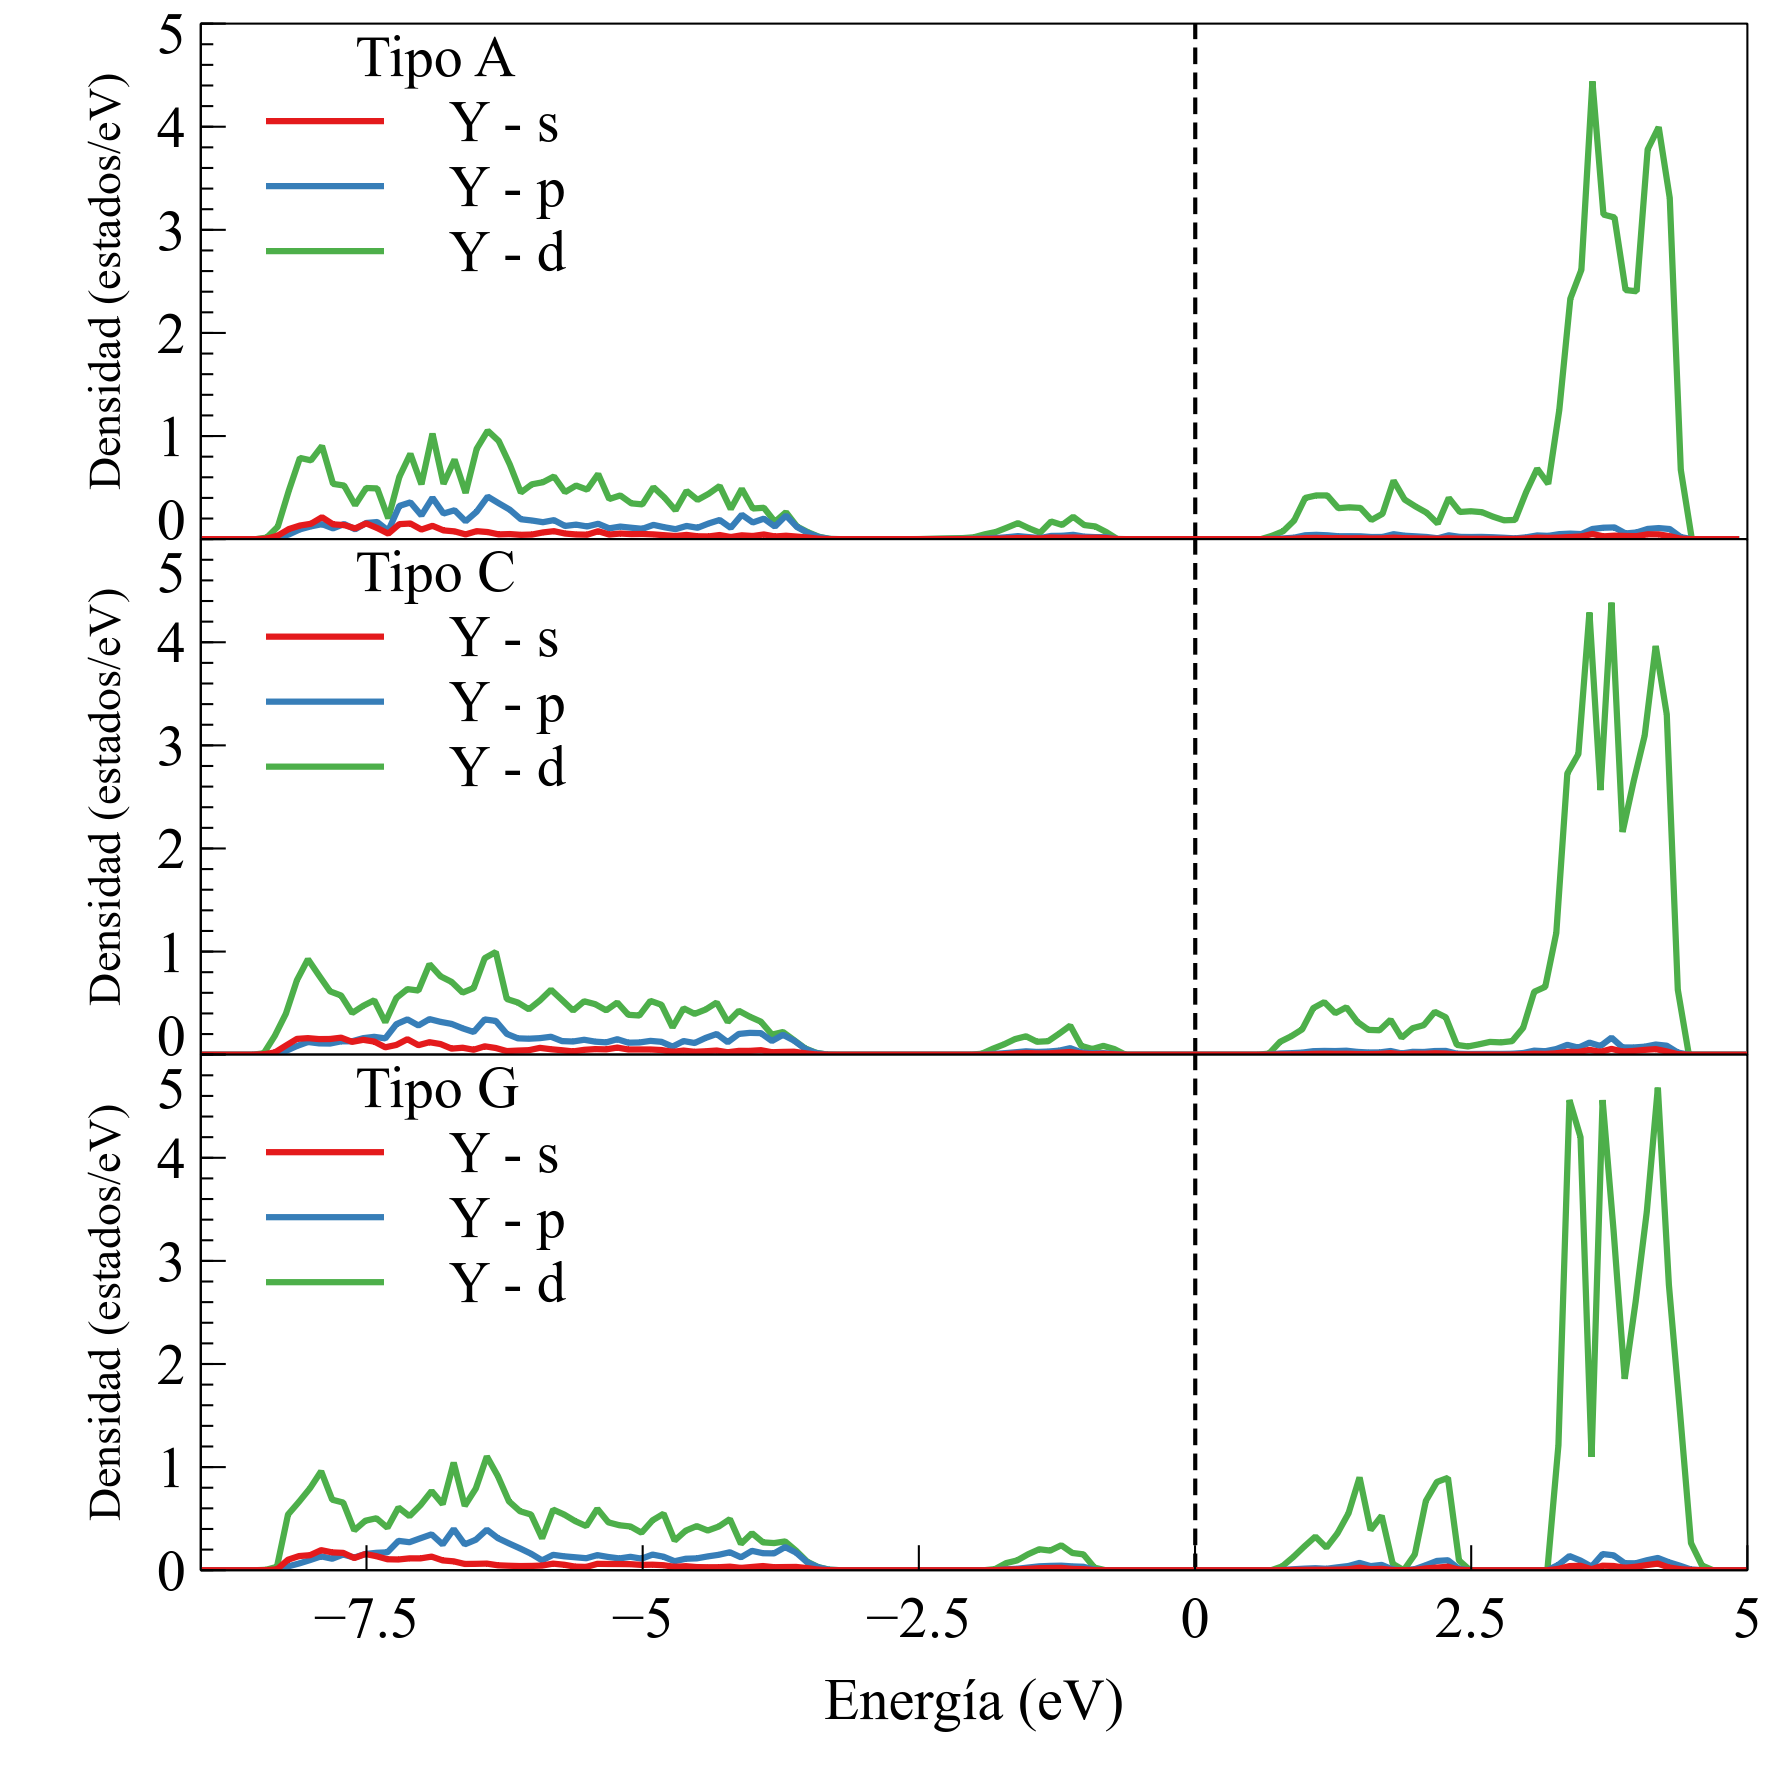
\includegraphics[width=1.0\textwidth]{contenido/resultados/img_resultados/YCO_Y_tipos.png}
        \caption{Densidad de estados parcial del itrio del $YCrO_{3}$.}
    \end{figure}
    \column{0.5\textwidth}
    \begin{figure}[H]
        \centering
        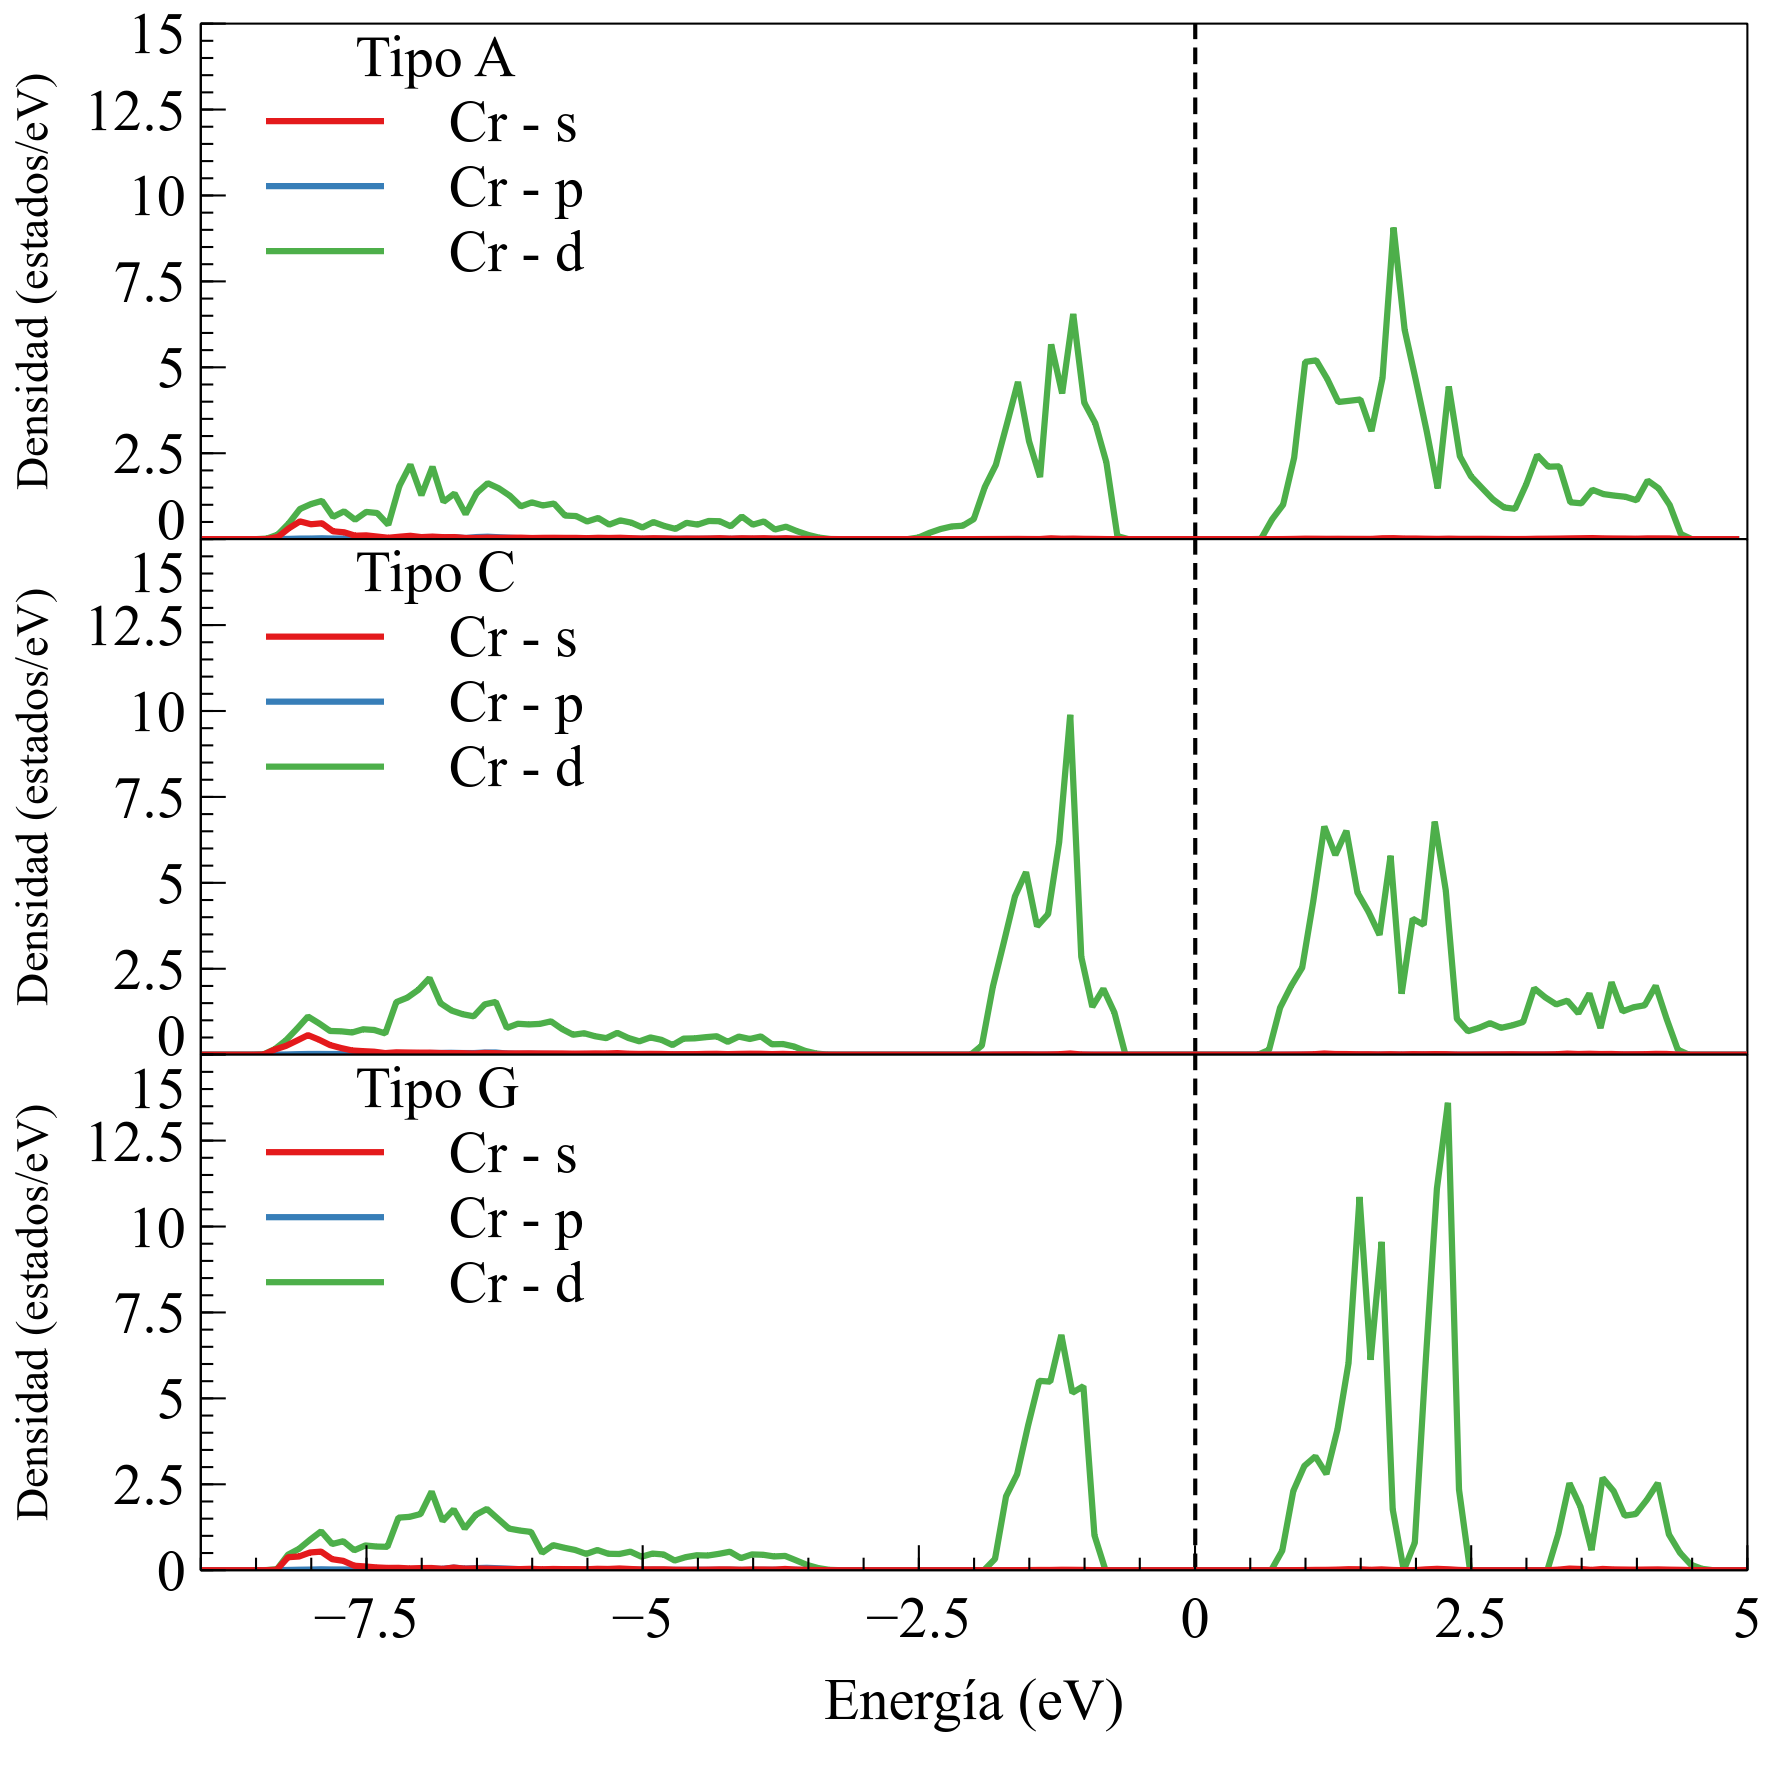
\includegraphics[width=1.0\textwidth]{contenido/resultados/img_resultados/YCO_Cr_tipos.png}
        \caption{Densidad de estados parcial del cromo del $YCrO_{3}$.}
    \end{figure}
\end{columns}
\end{frame}

\begin{frame}
     \begin{figure}[H]
    \centering
    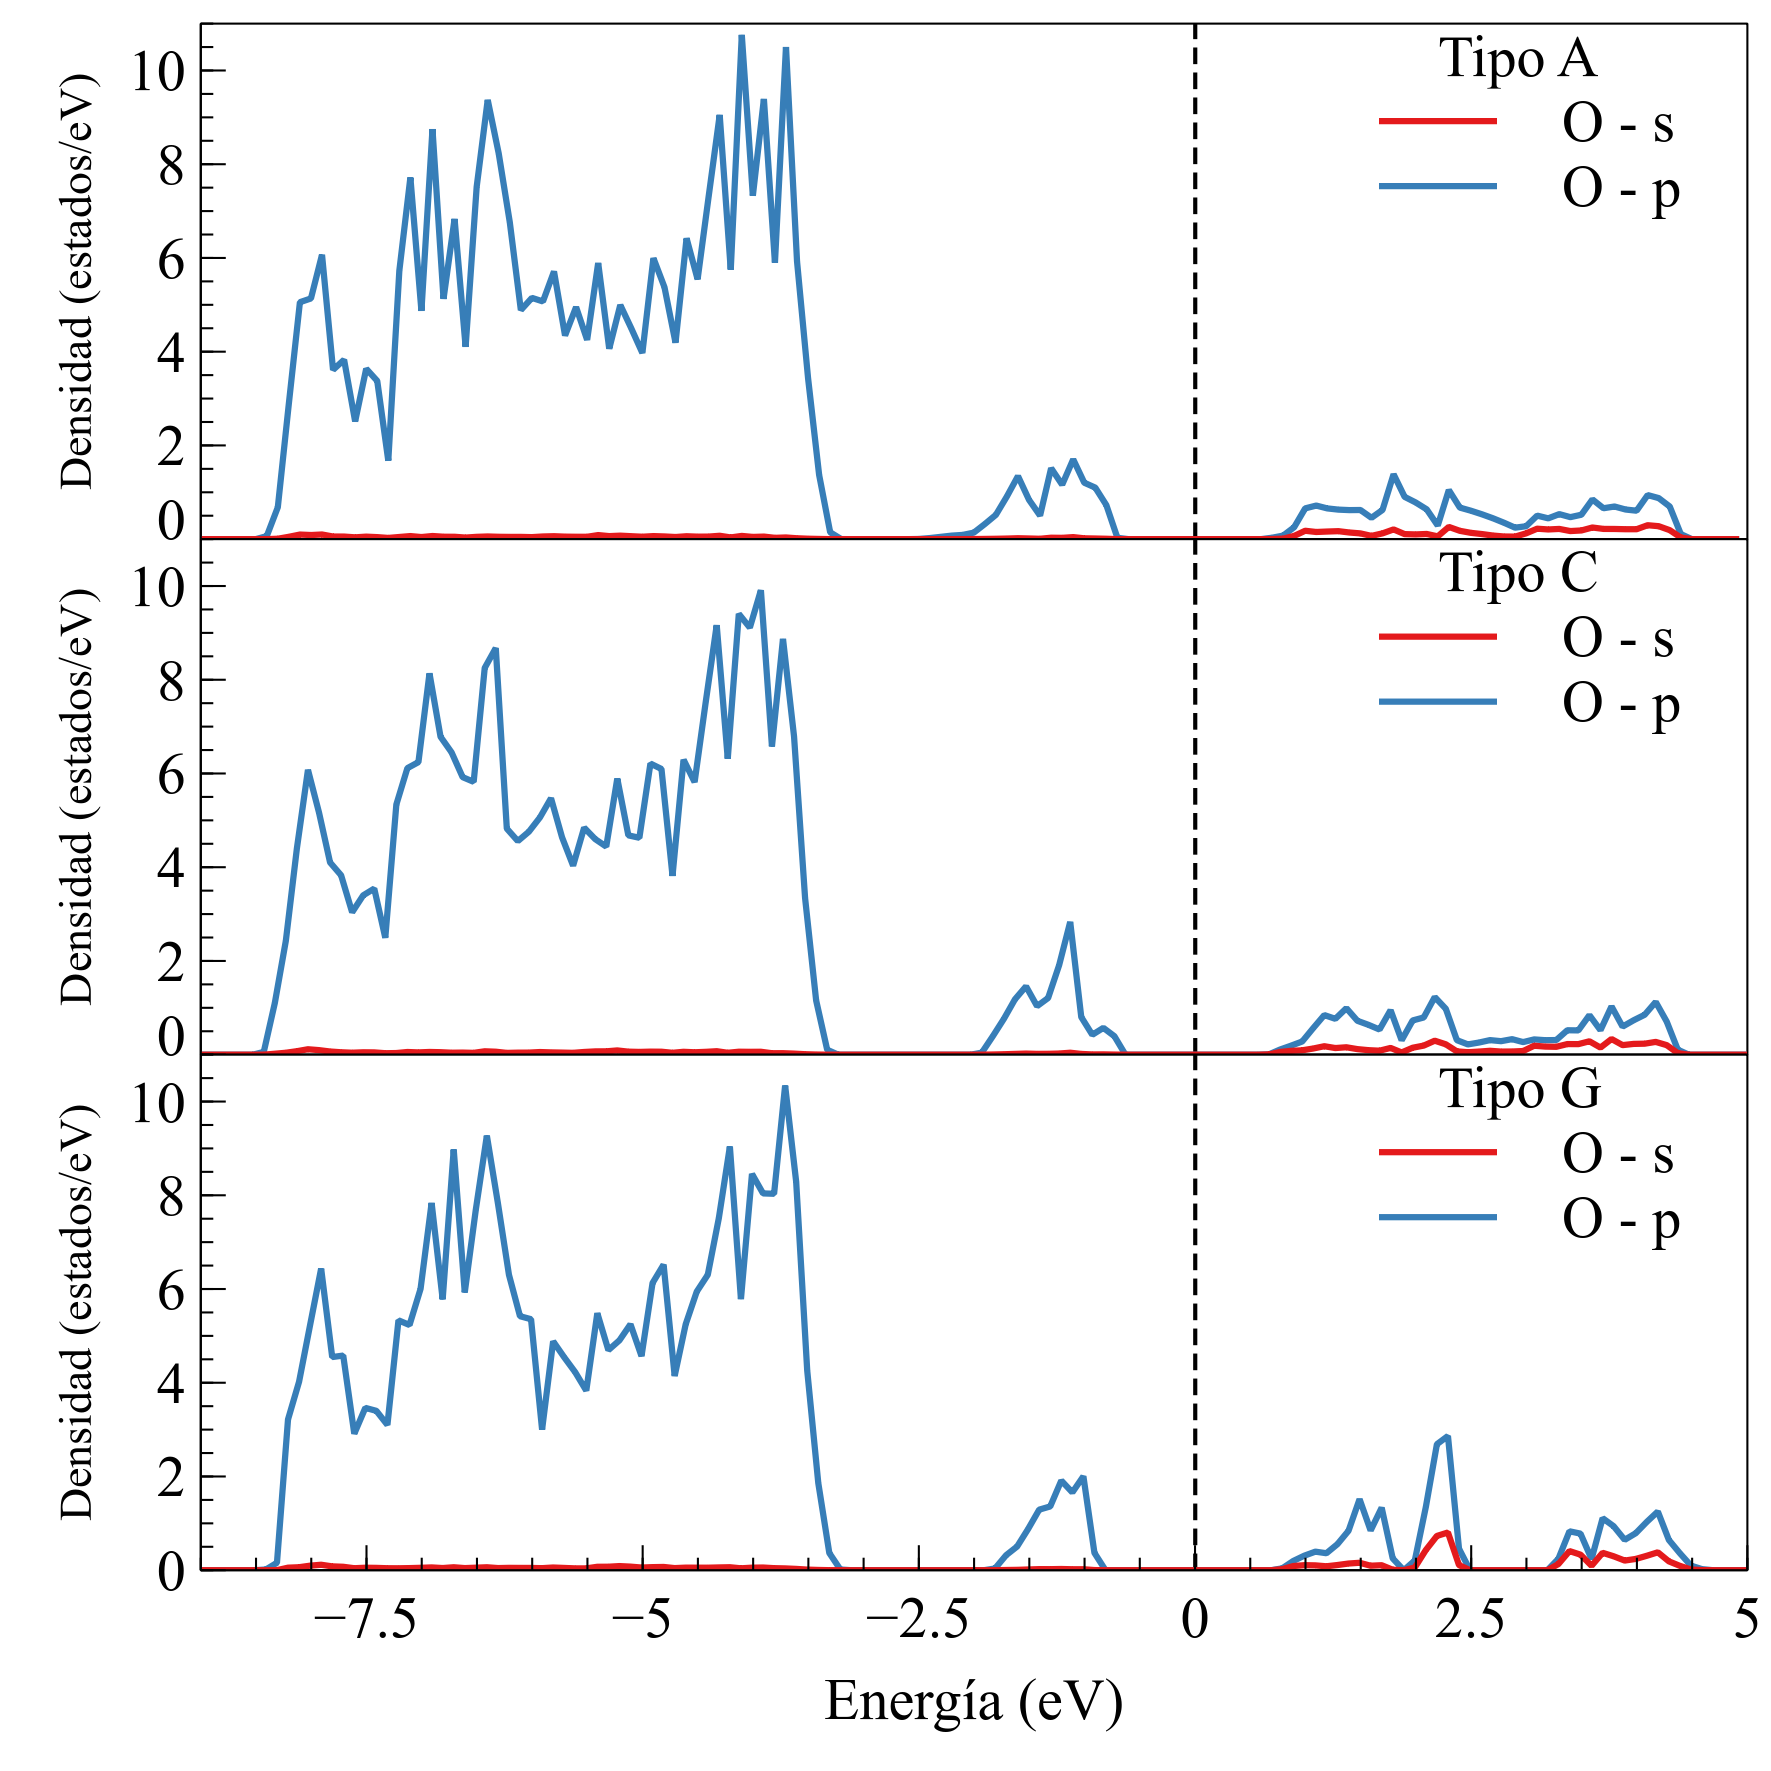
\includegraphics[width=0.5\textwidth]{contenido/resultados/img_resultados/YCO_O_tipos.png}
    \caption{Densidad de estados parcial del ox\'igeno del $YCrO_{3}$.}
    \end{figure}
\end{frame}